\graphicspath{{images/}}

\section{Discussion}
\label{sec:discussion}

% Over a whole plate, the competition model fit P15 with similar
% closeness as the logistic model, and with greater closeness in the 3x3
% zone studied (Figure~\ref{fig:comp_fit_plate} and
% \ref{fig:P15_zone_fit}). This is despite using a 387 rather than
% parameters, and having to include noisy edge cultures in the fit.

On average, the competition model fit internal cultures of P15 worse
than the logistic model: objective function value was 0.194 vs 0.155
(Table~\ref{tab:P15_obj_fun}). However, for the two fastest growing
cultures in a 3x3 zone studied in more detail, the competition model
fit much better than the logistic model because logistic model
objective function values were particularly high
(Figure~\ref{fig:P15_zone_fit}). I am yet to confirm that this trend
carries across the plate, but it is likely that the logistic model
performed better in regions where there were more slow growing
cultures and less difference in growth between neighbours. It would be
unsurprising if the independent model better fit slow growing cultures
because it is more flexible, and edge cultures were greatly affected
by noise due to the low inoculum density used.
% The independent model fits all cultures independently with three
% culture level parameters, whereas the competition model fits all
% cultures collectively with only one culture level parameter.
Estimated parameters might be less accurate despite the closer
fit. Noise from slow growing cultures will also have affected
competition model fits for fast growing cultures through plate level
parameters and neighbour interactions.
% For next section: use higher inoculum density.

Estimates from edge cultures are discarded due to noise from
reflections off plate walls. Unlike the logistic model, the
competition model must fit these cultures. For the fit of P15, edge
cultures contributed 70\% of error in objective function value despite
making up only 20\% of cultures (Tables~\ref{tab:P15_obj_fun} and
\ref{tab:corner}). This will have affected all parameter estimates
because cultures were fit collectively. However, it will have most
greatly affected cultures neighbouring an edge. A two \(N(0)\)
parameter model improved the fit of these cultures
(Table~\ref{tab:corner}) and might also have improved the accuracy of
estimated parameters.
% For next section: leave edges empty; use smaller zones with empty
% edges.
Considering the above effects and the fewer number of parameters used
(387 vs 1152) the closeness of fit of the competition model is fairly
good. Below I discuss differences in estimated parameters to discern
whether one model made more reliable estimates.

% Fits of the competition model (Figures~\ref{fig:comp_fit_plate} and
% \ref{fig:P15_zone_fit}) use less parameters than fits of either the
% logistic or generalised logistic model from the QFA R package
% \citep{qfa2016}. The competition model must also include noisy edge
% cultures, which contribute disproportionately to the objective
% function, in collective fits
% (Section~\ref{sec:treatment_of_boundaries}). Despite this, the fit of
% the competition model is of similar quality to fit of the logistic
% model over a whole plate and better in the 3x3 zone studied
% (Figure~\ref{fig:P15_zone_fit}). In particular, the competition model
% provided a much better fit to the fast growing cultures in
% Figure~\ref{fig:P15_zone_fit}. If the source of competition is
% nutrient diffusion between fast and slow growing cultures, competition
% effects are likely to be greater for these cultures. The competition
% model may be correcting for this.

For P15, the distribution of logistic model \(r\) estimates is
bimodal, whereas that of the competition model is unimodal
(Figure~\ref{fig:P15_correlations}). It is possible that the true
distribution is bimodal because \citet{Addinall2011} selected
deletions suspected to have large positive and negative interactions
with the query mutation. Nevertheless, repeats of the same strain are
split between the gap in the logistic distribution; it appears that
some deletions are acting as both enhancers and suppressors, but not
as neutrals. It is possible that the split is an artefact of the
heuristic checks conducted by QFA R, or caused by a relative
acceleration and deceleration of fast and slow growing cultures due to
competition. If the latter case is true, the competition model might
have corrected for it.
% Below could wait for future work.
It is important to investigate the cause of the bimodal distribution
because it will affect the significance given to genetic interactions
(see e.g. \citet{Addinall2011}).


% In the correlation of logistic and competition model \(r\) estimates
% for P15 (Figure~\ref{fig:P15_correlations}), there is a split in the
% distribution of logistic model \(r\) estimates, but not competition
% model \(r\) estimates. It is possible that the distribution of median
% \(r\) for strains selected by \citet{Addinall2011} does have such a
% split distribution. However, repeats of many individual strains fall
% in either group but not in the gap. This is evidenced by the positions
% of medians in the gap (red). It seems unlikely that the same split
% exists in the distributions of \(r\) for repeats of each strain and at
% the same value. It is possible that the split is either an artefact of
% the heuristic checks conducted by QFA R fits of the logistic model for
% slow growing strains \citep{qfa2016}, or caused by a relative
% acceleration and deceleration of fast and slow growing cultures due to
% competition between neighbours. If the latter case is true, the
% competition model appears to correct for it. It is important to
% investigate the cause of the split distribution because it will affect
% the significance given to genetic interactions in QFA studies (see
% e.g. \citet{Addinall2011}).

Competition model fitness ranking of deletions on P15 is similar to
the published logistic model ranking from \citet{Addinall2011} for the
fastest and slowest growing strains
(Figure~\ref{fig:comp_vs_log_ranking}). Both models also agree with
rankings from independent spot tests for these strains
\citep{maringele2002exo1,zubko2004exo1,Holstein20141259,foster2006mrx}.
Middle rankings, however, disagree between models, and Spearman's Rho
between \(MDR\) estimates for all cultures is just
0.635. Unfortunately, I lack independent data for these strains to
discern which model is more accurate.

The competition model was more precise for the majority of strains (36
out of 50), but less precise for the 11 fastest growing (see
Figure~\ref{fig:COV}). The fastest growing cultures are not split
across the gap in the logistic model distribution. Although it is
ultimately the accuracy of the distributions that matters, it is,
nevertheless, reasonable to expect the better model to make more
precise estimates. Features of each model could contribute to the
differences in precision. The logistic model fits cultures
individually so it can be more precise for fast growing cultures which
are less affected by noise. Conversely, the competition model fits
cultures collectively, worsening the precision for fast growing
cultures but improving the precise for slow growing cultures.
% noise dominated cell observations from slow growing cultures
% will affect collectively fit competition model parameters. This does
% not affect logistic model estimates because cultures are fit
% individually.
The higher precision for slow growing strains in the competition model
could be entirely due to collective fitting rather than accuracy of
the model. Similarly the higher precision for fast growing strains in
the logistic model could be due to a failure to account for
competition. Although improved with the competition model, the
precision of estimates for the slowest growers is still much lower
than for the fastest, so the power to infer genetic reactions might
not be dramatically improved.


Fitting the logistic model to slower growing cultures requires
heuristic checks to correct for confounding between \(r\) and
\(K\). The QFA R implementation appears to have some issues. The
strains \textit{est1\(\Delta\)} and \textit{rad50\(\Delta\)} and are
outliers in Figure~\ref{fig:P15_correlations} and this causes a
dramatic change in ranking between logistic model \(r\) and \(MDR\)
(Figure~\ref{fig:comp_vs_log_ranking}). I confirmed that these were
weak growing strains by visual inspection of the raw QFA images. High
\(r\) and low \(K\) have been erroneously fit to both. This is
corrected for when converting to \(MDR\) which agrees with the
competition model ranking and independent validation for
\textit{rad50\(\Delta\)} \citep{zubko2004exo1}. \(MDR\) is more
similar to the fitness measure (\(MDR \times MDP\)) used in the
original analysis by \citet{Addinall2011} so this is unlikely to have
affected their results. For other cultures it appears that
encroachment of fast growing cultures into neighbours is affecting
cell density estimates made by Colonyzer \citep{Lawless2010}. If
repeated, the plate from \citet{Addinall2011} should be run with a
lower concentration of nutrients in the agar so that the stationary
phase is reached before cultures start to merge.

I looked at plate images of P15 to investigate other discrepancies.
%  ~\textit{mre11\(\Delta\)} is a weak growing strain
% \citep{zubko2004exo1,Addinall2011} which was misclassified as healthy
% by the competition model when I was using mean values (not shown) but
% not the logistic model. One repeat contained unusual heterogeneity,
% which may be natural or the results of contamination, and may explain
% the discrepancy. I corrected for this by taking median values in Figure~\ref{fig:comp_vs_log_rankinkgsattempted to correct for this issue by taking the median with partian
% nmedian rather than mean values.
\textit{hap4\(\Delta\)} appears to be much healthier than
\textit{zrt3\(\Delta\)}, which agrees with the competition model but
not the logistic model (Figure~\ref{fig:comp_vs_log_ranking}). The
estimate for \textit{zrt3\(\Delta\)} is more precise for the logistic
model than for the competition model (Figure~\ref{fig:COV}). However,
this does not confer greater accuracy to either model because the
opposite is true for \textit{hap4\(\Delta\)} estimates. Unfortunately,
independent data for validation of the middle strains is not available
so it is difficult to draw conclusions.

Recent work Herrmann and Lawless suggests that direct measurements of
\(C(0)\) may not be reliable due to heterogeneity between cells in the
same inoculum; many cells do not grow and only the fastest growing
cells contribute significantly to the final population. A plate level
\(C(0)\) also seems inappropriate but having extra parameters for the
starting cell density of each culture is undesirable. Only a small
amount of nutrients is used when cultures are small. Therefore, early
timepoints could be discarded and \(C(0)\) could be measured when
populations have already undergone several divisions. QFA inocula use
cells taken from the stationary phase where there might be more
heterogeneity \citep{bergkessel2016}. It may be possible to increase
the precision of fitness estimates by taking inocula from the
exponential growth phase or using a higher starting density to average
out effects.

The Stripes and Filled plates used a higher inoculum density and had
very few noise dominated cultures. Compared to P15, this would have
reduced noise in collectively fit competition model estimates and
would not have required heuristic checks to be employed for the
logistic model. This may therefore be a fairer comparison than P15. It
would be informative to repeat P15 with an inoculum density at a
detectable level so that the precision of competition and logistic
model estimates can be compared in the absence of noise dominated
cultures. However the competition model struggled to find a global
minimum for the Stripes and Filled plates, which had higher inoculum
densities. Therefore, fitting would first need to be improved.
% Correlation of fitness estimates between plates in
% Figure~\ref{fig:r_correlations}a was similar for both models. This is
% despite not finding global minima with the competition model. However,
% correlation between models for the same plate in
% Figure~\ref{fig:r_correlations}b is poor. (Could definitely do with
% P15 correlations to compare).
There are issues with validation of both models
(Figure~\ref{fig:stripes_validation}); the logistic model does not
account for differences between plates at all and the competition
model overcorrects. As I lack independent data for validation it is
difficult to decide which to believe.
% (Unfortunately, the Stripes and Filled plates have few repeats so I
% could not study the reliability of estimates on the same plate. (I
% believe that we have more issues with accuracy than precision anyway).
In any case, it is clear that the competition model could be improved.


\subsection{Future work}

The split in the distribution of logistic model \(r\)
(Figure~\ref{fig:P15_correlations}) may offer a useful way to the
compare the logistic and competition models. Firstly, P15 could be
repeated using a higher inoculum density to eliminate the possibility
that the heuristic checks of the QFA R package are responsible for the
split. If the split still exists in only the logistic model, then the
strains could be grown in independent conditions, either isolated on
solid agar (diffusion still an issue) or in liquid cultures, where the
models are equivalent. If the split does not exist in the independent
distribution, then we may favour the competition model for QFA
plates. This will also depend on how well competition model estimates
agree between the two conditions.

% For the Stripes and Filled plates, the competition model was fit to 15
% cell measurement values taken from a spline, whereas the logistic
% model was fit to all timepoints. A little more work is required to
% compare the quaility of fits at these higher inoculum densities; I
% need to resimulate both models using estimated parameters and compare
% to the observed timepoints using the same objective function. With
% fewer noise-dominated cultures than in P15, the competition model fit
% may have improved.

I was unable to find global minima using a gradient method to fit the
competition model (Sections~\ref{sec:P15_fit} and
\ref{sec:cross_plate_val_results}). I began work on a genetic
algorithm method of solving but lacked time to complete this. I did
however find that, with fixed plate level parameters, it is possible
to reliably return \(b_{i}\) with a gradient method
(Figure~\ref{fig:comp_fit_fixed_plate_level}). This offers the
potential to use a hierarchical genetic algorithm where candidate
plate level parameters are fixed in gradient fits of culture level
parameters \(b_{i}\). Alternatively, a pure hierarchical genetic
algorithm may work (i.e. where \(b_{i}\) are also evolved). A
hierarchical Bayesian approach to fitting the competition model,
similar to that of \citet{Heydari2016}, used to fit the logistic
model, could also return global minima but might be slow. Current best
fits, which are different local minima, have well correlated fitness
rankings (Table~\ref{tab:Filled_best_fits}) and make similar
overcorrections for competition
(Figure~\ref{fig:stripes_validation}). This suggests that there is a
more fundamental issue with the model.

It would be informative to validate the independent limit of the
competition model to determine whether a mass action approximation is
valid and whether it is correct to ignore the effect of metabolism on
nutrient density. I suggest to validate first in liquid cultures,
where the assumption of a well stirred mixture is more valid, and then
attempt to validate for single cultures grown on agar, which more
closely resembles QFA. Growth on a surface has a lower dimensionality
and may be diffusion limited so a fractal kinetics model may be
required \citep{Kopelman1988,savageau1995}. Nutrients (sugars,
nitrogen, etc.) in QFA agars are of a standard composition, designed
to reduce the excess of any single nutrient \citep{Addinall2011}. It
would be helpful to know and control the identity of the limiting
nutrient using a different formula of agar. With nitrogen, rather than
sugar, as the limiting nutrient, we are less likely to have to model
metabolism.

Estimates of the nutrient diffusion constant \(k\) were fairly high,
such that nutrients diffused readily between neighbours and were
nearly depleted when growth stopped. It may be that growth becomes
limited by the diffusion of nutrients through agar before all
nutrients are depleted and that nutrients are not well approximated as
being evenly distributed across the spatial scales that we
model. Using a finer grid could reduce the overcorrection seen in
Figure~\ref{fig:stripes_validation}. \citet{Reo2014} use the diffusion
equation with Neumann and Dirichlet boundary conditions to simulate
nutrient dependent growth of a single bacterial culture on a pertri
dish in two-dimensions. They create a sink for nutrients from culture
growth and equate the flux of nutrients through culture area with the
rate of increase in culture size. They model culture area as varying
and keep culture density constant. This model could be adapted for QFA
by keeping culture area constant and allowing culture density to
vary. A mass action kinetic model of reaction~(\ref{eq:reaction})
could be used for culture growth and the nutrient sink. It would be
computationally challenging to use such a detailed model to fit a
whole plate but simulation could be very informative.

If we find that competition for nutrients is not responsible for the
interaction between neighbours, for instance if growth becomes limited
by diffusion of nutrients in the agar before nutrients from neighbours
can be accessed, then we could instead model signalling by ethanol
poisoning \citep{fujita2006}. Signal diffusion may be modelled as we
have done for nutrient diffusion
(\ref{eq:competition_model},\ref{eq:diffusion_reaction}) so much of
the code could be reused. If there is any combination of competition,
metabolism, signalling, or arrest contributing significantly to
differences in the growth of cultures and the interaction between
neighbours, then it will be difficult to separate them when fitting a
model to data. We may have to develop ways to calibrate effects in
isolation and use this information when fitting to high-throughput
data. We only have observations for cells.

\subsection{Improvements and other recommendations}

It is quicker to fit to small zones of a plate but, as these have a
larger proportion of edge cultures, boundary conditions become
important. Gathering QFA data from smaller arrays grown in isolation
would help to speed up the development process.
\\\\
Each culture is surrounded by a different group of neighbours with
different growth constants \(b_{j} \in \delta_{i}\)
(Figure~\ref{fig:comp_model_schematic}). The imaginary neighbour guess
(Section~\ref{sec:guessing_b}) could be improved by using a range of
\(b_{f}\) values to fit each culture and selecting \(b\) from the best
fit. \(k\) is the last parameter to be guessed. Rather than using the
linear relationship between variance in final cell measurement and
\(k\), which may not hold for large values of \(k\), it would be
better and just as quick to guess a value of \(k\) by fixing all other
parameters as the guesses and fitting the competition model to
data. It would also be good to compare guesses from the imaginary
neighbour model with those from the logistic model. Even with an
improved guess, I suspect, based on the closeness of current fits
(Figure~\ref{fig:P15_zone_fit}), that a gradient method will still
fail to find global minima.
\\\\
Edge cultures must be included in data when fitting the competition
model and this contributed significantly to objective function values
(see Table~\ref{tab:corner}). Noise might be better dealt with by
leaving edge cultures empty. A different treatment of boundaries could
also be used by modelling empty cultures outside edges rather than the
approach in Section~(\ref{sec:fitting_comp}).
% The design of the stripes validation experiment could be
% improved. Rather than filling gaps with cultures not present on the
% stripes plate, and for which we have no \(b\) estimates, we could fill
% with repeats of the cultures already present on the stripes
% plate. (I'm not sure it makes any difference actually whether we
% validate from one direction to the other). It would also have been
% helpful to have repeats to study differences in COV between the
% competition and independent models.
\\\\
In order to make sure that competition effects were present in data,
E. Holstein (personal communications) made a dramatic change between
the Stripes and Filled plates. I could have first validated the model
against a smaller change, by varying between slower and faster growing
cultures rather than no cultures and very strong growing cultures. If
the model works well between such plates, it may work well for the
majority of QFA experiments which typically have smaller differences
between cultures than the data we studied. We could also have
calibrated and validated from the Stripes plate to the Filled plate
(i.e. in both directions) if the same genotypes had been inoculated in
the extra columns of the Filled plate. If we did want to test the an
extreme case, we could have inoculated fast growing cultures next to
certain strains and not others to try to induce a change in ranking
for which the competition model might compensate better than the
logistic model.
\\\\
It is desirable to have a mechanistic model including nutrient
dependent growth so that we can use a plate level \(N(0)\) and
eliminate the dependence on heuristic checks.
%%%%%%%%%%%%%%%%%%%%%%%%%%%%%
%%%%%%%%%%%%%%%%%%%%%%%%%%%%%
%%%%%%%%%%%%%%%%%%%%%%%%%%%%%
%%%%%%%%%%%%%%%%%%%%%%%%%%%%%

% %% insert this somewhere %%%%%%%%%%
% //Noise affecting competition model//

% I also had some thoughts about why the competition model might have
% higher variance. The competition model has to deal with noise of the
% slowest growing cultures which affects both plate level parameter
% estimates and the b estimates of faster growing
% neighbours. I.e. sharing plate level parameters gives us more
% information about slower growing cultures but adds noise to our
% estimates of faster growing cultures. For the logistic model, each
% growth curve is fit independently and so fast growing cultures are
% less affected by noise and may have less variance than competition
% model estimates. Conversely slow-growing cultures are dominated by
% noise and this requires us to use heuristic checks (accuracy is
% actually affected more than precision). This may be why we see more
% variance in the b estimates of fast growing cultures from the
% competition but less for medium and slow growing (probably also less
% overall). If we had a plate with no very slow growing cultures
% dominated by noise perhaps we would see less variance in the fastest
% growers from the competition model. We could probably use the filled
% plate to check this.

% %%%%%%%%%%%%%%%%%%%%%%%%%%%%%%%%%%%

% In light of heterogeneity. For independent fits may start with
% inoculum density below the level of detection and take time zero the
% time when cells first reach some observable level. I.e. different
% \(t_{0}\) for each culture.


% (Wait until discussion: Recent work by Herrmann and Lawless - issues
% with plate level \(C(0)\) - Could approximate cells as not
% starting to grow until levels become detectable at \(t_{i}\) (OK if
% assume only small diffusion before this point)).


% %%%%%%%%%%%%%%%%%%%%%%%%%%%%%%%%%

% Possible to have fast nutrient limited diffusion without nutrinet
% competition and poisoning by ethanol. Separable.

% %%%%%%%%%%%%%%%%%%%%%%%%%%%%%%%%

% Fitness ranking from competition model fits may be better than from
% logistic model fits (Will comparing stripes rankings reveal
% anythin?). However, we cannot quantitatively compare fitness estimates
% between plates because we are not finding global minima. Work has
% begun to develop a genetic algorithm to do so. I am not convinced that
% this will succeed because growth is systematically overestimated when
% we move from the filled to striped plate for all of the current best
% parameter solutions. This suggests an issue with the modelling
% approach; below I suggest ways in which this could be improved. In
% any case, qualitative cross-plate validation using order of fitness
% ranking may still be better (for the competition model).


% The first thing to notice about QFA data - from P15, the striped
% plate, and the filled plate - is the characteristic endpoint in growth
% on each plate (experiments could be designed to study variation in
% timescales over regions of a plate by inoculating cultures in columns
% left-to-right according to fitness). This suggests a plate-level or
% region-level growth-limiting effect.
% //
% Could this conceivably be an experimental limitation such as the
% drying out of an agar plate over time?
% //
% Comparison of the striped and filled data, shows that cultures grow
% larger when neighbours are removed and this suggests a direct
% interaction between cultures. The strongest candidates are competition
% for nutrients and growth limiting signalling such as ethanol
% poisoning. It is possible that other growth limiting effects may exist
% and could confound any attempt to fit a model which accounts for just
% one of these. It makes sense to investigate each likely effect in turn
% to determine its contribution and to start by validating the
% independent limit.

% There is a characteristic timescale for the cessation of growth which
% I believe to be caused by an interaction between cultures.

% The an experiment to test the length-scale of the competition interaction
% could inoculate a gradient of fast to slow growing cultures across a
% plate and observe local differences in endpoint.


% Spots can grow after a long time. Must be nutrients remaining or an
% encroachment? I have an image for the stripes plate showing cultures
% growing and believe after a very late stage. I need to check the data
% images but this may just be encroachment of another culture.
% \graphicspath{{images/stripes/}}
% \begin{Figure}
%   \centering
%   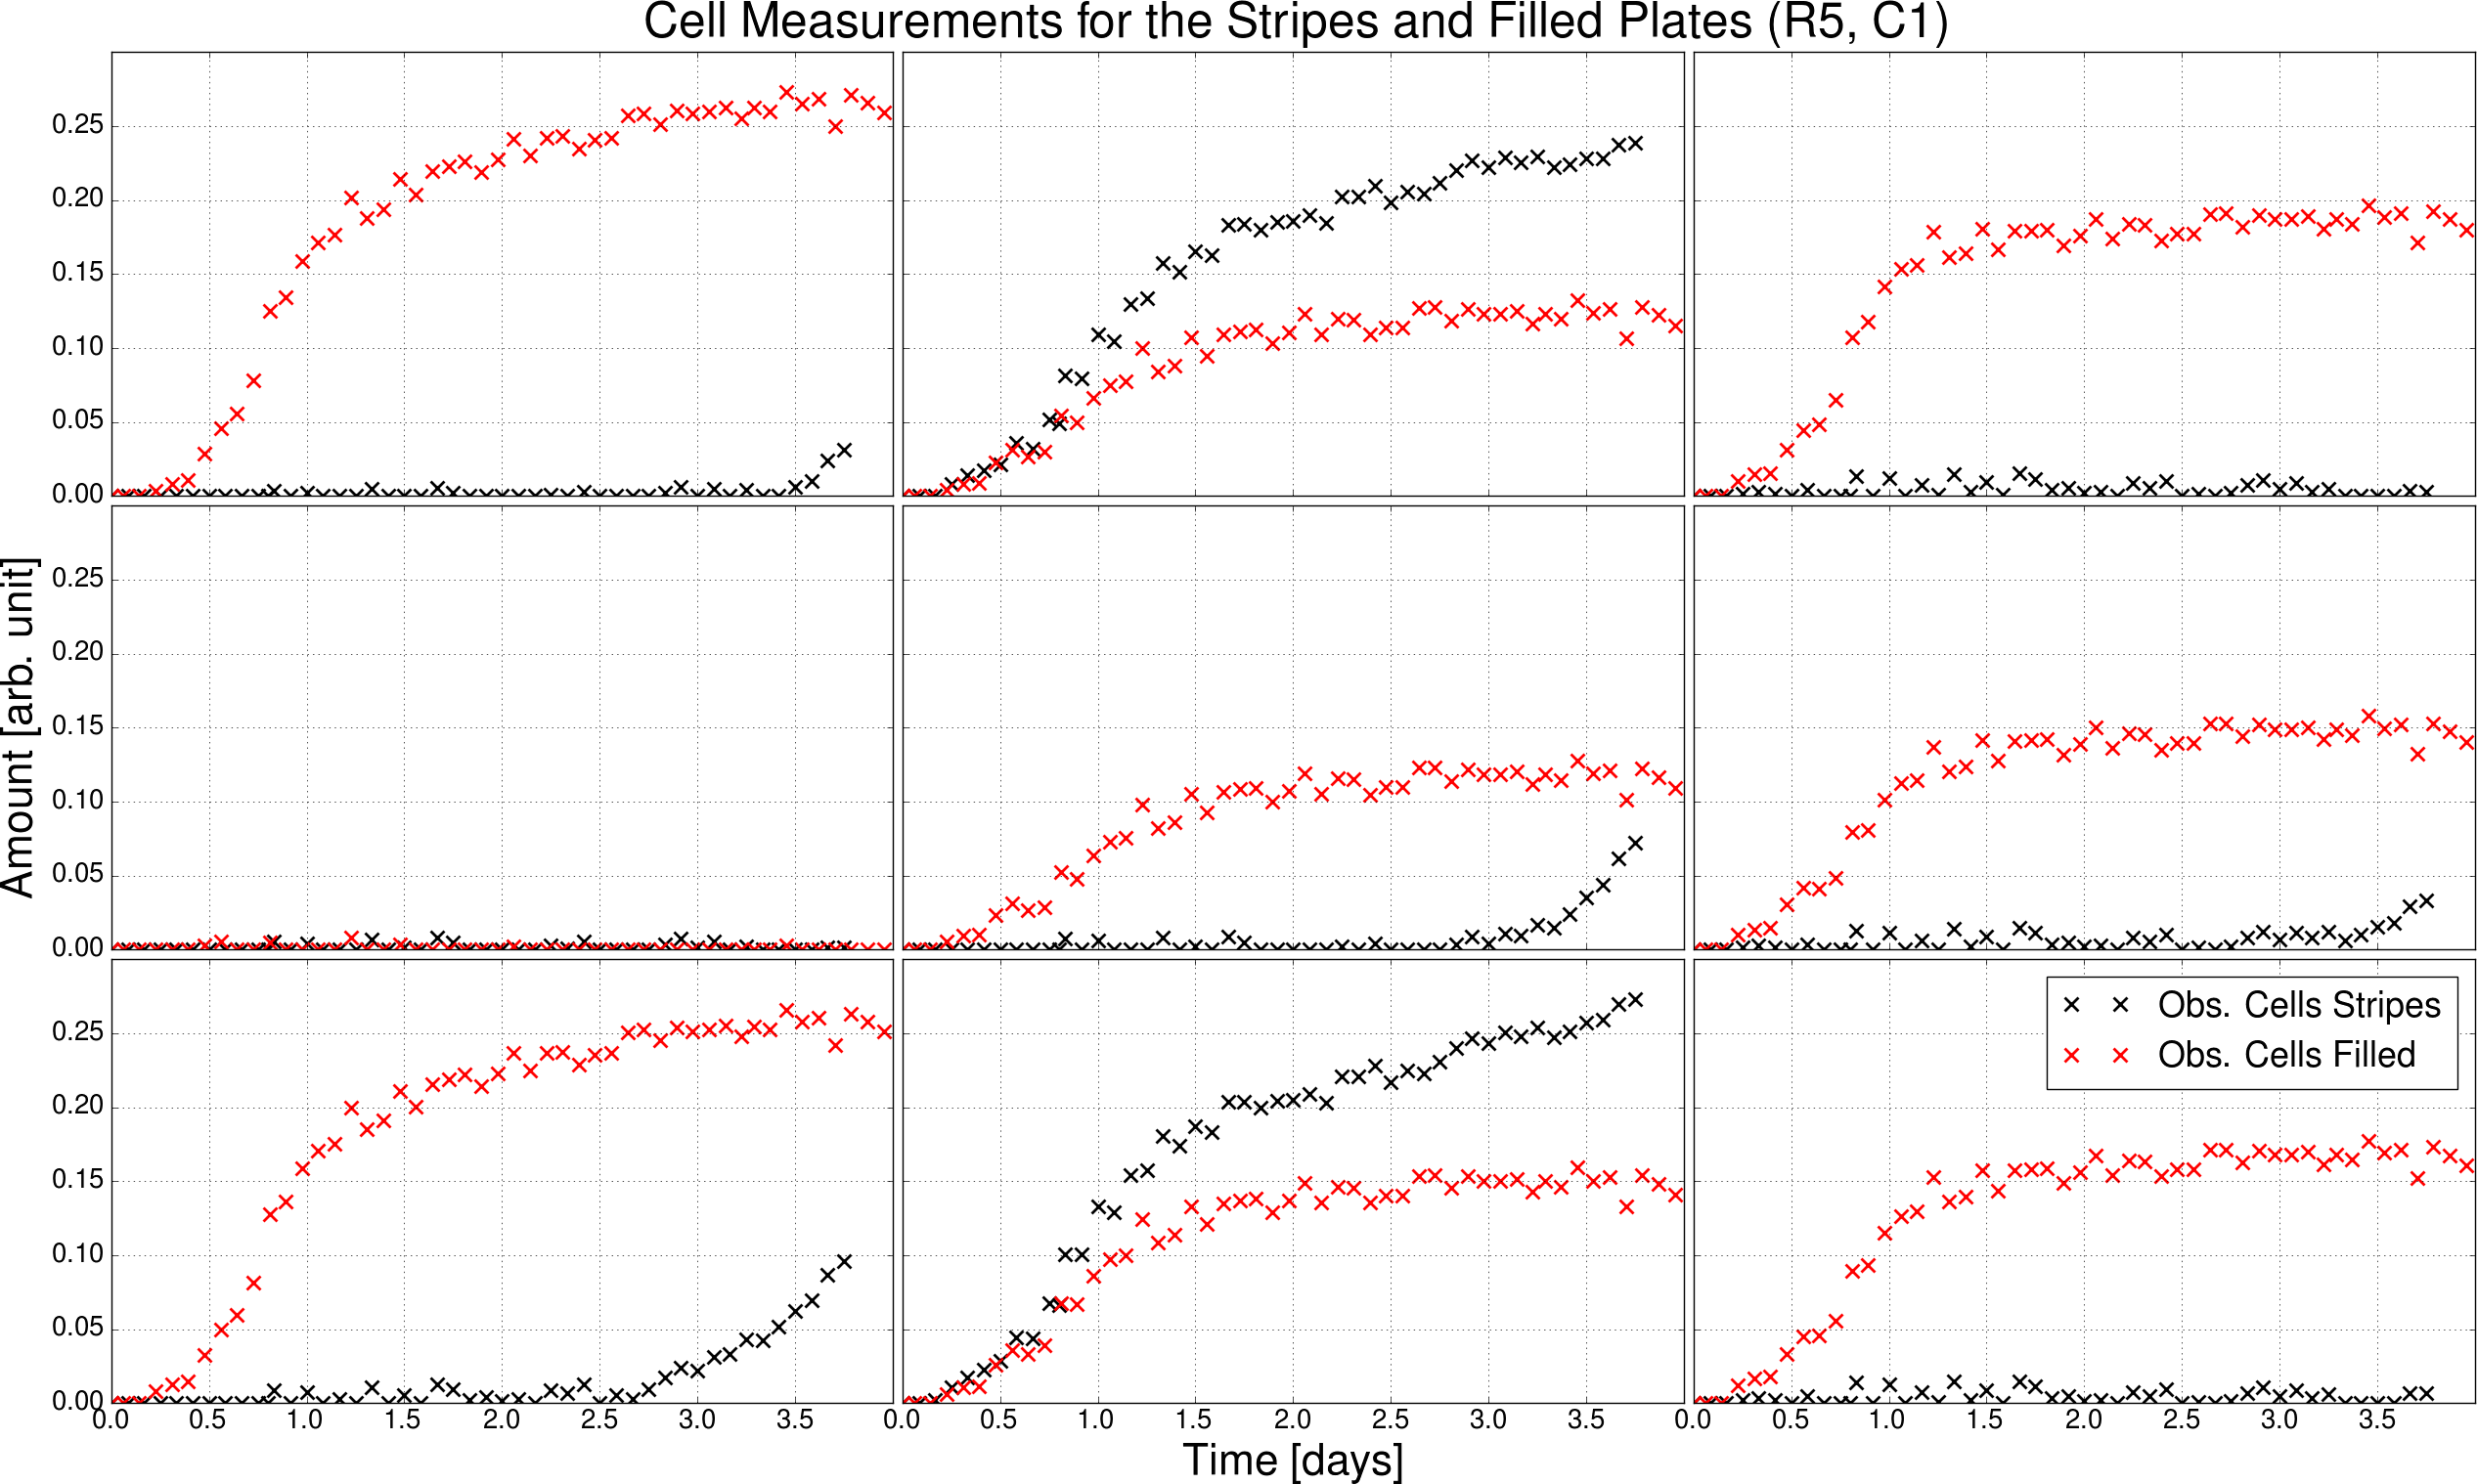
\includegraphics[width=\linewidth]{final/c_meas_r5_c1}
%   \captionof{figure}{Observed cells for (R5, C1) 3x3 zone of Stripes
%     and Filled plates showing (for Stripes data) slow growing cultures
%     starting to grow after faster growing cultures have reached the
%     stationary phase.}
%   \label{fig:kn_guessing}
% \end{Figure}


% We have only studied data where cultures are grown in an array on
% solid agar where we cannot validate the independent limit. In this
% limit, our model says that nutrients can only be converted to cells
% and all cultures starting with the same amount of nutrients will reach
% the same final cell density. This ignores metabolism which may differ
% between strains. Cell arrest could also limit growth (and this may
% occur in different strains at different rates). If present,
% differences in such effects could account entirely for differences in
% final cell density. However, they are unlikely to be the only effect,
% because this would not lead to the observed characteristic endpoint in
% growth. Using one-culture spot tests (in a perti-dish on ager?) or
% liquid cultures we can grow cultures independently and validate the
% independent limit. A current issue with methods for estimating
% fitness, is that identical strains grow differently on agar or in
% liquid culture leading to different fitness rankings (cite). This
% problem need not affect our validation as we can simply define a
% culture to have different parameters for growth in either medium. A
% greater difference may be caused by the dimensionality of the
% environment. Mass action kinetics is derived for reactions in a
% three-dimentsional (gas or fluid?) (Guldberg and Waage C.M. Guldberg
% and P. Waage, Studies Concerning Affinity, C. M. Forhandlinger:
% Videnskabs-Selskabet i Christiana (1864), 35) and this approximation
% is more valid for liquid cultures than for cultures spotted onto a
% surface. I suggest to study first the more ideal case of liquid
% cultures and later see if the model holds for cultures grown on a
% surface. If it does not, it may be necessary to use a fractal kinetics
% model (I have references for this from the proposal) or, if the
% reaction is diffusion limited, consider a more detailed model of
% nutrient diffusion.

% // Model equations for metabolism.//

% Our model splits the agar into a grid with volume discretised per
% culture. In the stripes validation, we overestimate the effect of
% diffusion when neighbouring cultures are removed. I believe that we
% are not accurately capturing the point at which growth becomes
% diffusion limited and that nutrients are well approximated as being
% evenly distributed withing the spatial scales that we model. A
% diffusion equation model could capture the local distribution of
% nutrients around a culture when the stationary phase is reached.  Reo
% and Korolev (2014) use the diffusion equation (with Neumann and
% Dirichlet boundary conditions) to simulate nutrient dependent growth
% of a single bacterial culture on a pertri dish in two-dimensions. They
% create a sink for nutrients from culture growth and equate the flux of
% nutrients through culture area with the rate of increase in culture
% size. They model culture area as varying and keep culture density
% constant. This model could be adapted for QFA by keeping culture area
% constant and allowing culture density to vary. A mass action kinetic
% model of reaction~(\ref{eq:reaction}) could be used for culture growth
% and the nutrient sink. Simulating or fitting this model could help us
% learn more about diffusion in QFA experiments. It is probably
% computationally unfeasible to use such a detailed model to fit a whole
% plate. However, if necessary, it may be possible to use a finer grid
% to increase compartmentalisation of nutrients to capture spatial
% heterogeneity in the distribution of nutrients around a culture and
% the effect of diffusion limited growth. This could extend the validity
% of the competition model over a larger range of variability in culture
% growth rates (for instance when some cultures are left empty and
% others are very fast growing.)

% It would also be useful to determine experimentally how nutrients are
% distributed throughout the agar at the stationary phase. Gaps could be
% left in an array of cultures and only inoculated once the stationary
% phase is reached. If they grow then nutrients remain. (Sill require
% simulations to see distribution across depth). This could be extended
% by growing a single column of identical strains and, after the
% stationary stage has been reached, inoculating identical strains on
% the same plate at different distances from the row.

% //Talk about an improvement to the imaginary neighbour model.//

% Nutrients (sugars, nitrogen, etc.) in QFQ agars are of a standard
% composition, designed to reduce the excess of any single nutrient
% (check QFA paper and cite). ((background) What is the nutrient?
% Nitrogen is only used to build molecules for new cells, whereas sugars
% are also used for metabolism.) For modelling nutrient limited growth,
% especially across plates, it would be useful to know the identity of
% the limiting nutrient and ensure that it is always the same. We could
% achieve this using a different formula of agar.

% The design of the stripes validation experiment could be
% improved. Rather than filling gaps with cultures not present on the
% stripes plate, and for which we have no b estimates, we could fill
% with repeats of the cultures already present on the stripes
% plate. (I'm not sure it makes any difference actually whether we
% validate from one direction to the other). It would also have been
% helpful to have repeats to study differences in COV between the
% competition and independent models. In order to make sure that
% competition effects were present in data, we made a drastic change
% between the stripes and filled plates. This provides a stern
% validation. The model assumes that competition effects are present
% whenever there is a difference in final cell amounts between
% cultures. We could have first validated the model against a smaller
% change, by varying between slower and faster growing cultures rather
% that none and very strong growing cultures. If the model works well
% between such plates it may work well for the majority of QFA
% experiments which typically have smaller differences between cultures
% than the data we study. If we did want to test the in an extreme case
% we could have inoculated fast growing cultures next certain strains
% and not others to try to induce a change in ranking for which the
% competition model might compensate better than the logistic model.

% //Signalling//

% If we find that competition for nutrients is not a significant effect,
% for instance if growth becomes diffusion limited before nutrients from
% neighbours can be accessed, then we could instead model signalling by
% ethanol as the interaction effect. This may be modelled similarly to
% how we are already modelling nutrient diffusion.

% //Signalling equation//

% If there is any combination of competition, metabolism, signalling, or
% arrest contributing significantly to differences in the growth of
% cultures and the interaction between neighbours then it will be
% difficult to separate them when fitting a model to data. We may have
% to develop ways to calibrate effects in isolation (e.g. by
% adding/measuring ethanol?) and use this information when fitting to
% high-throughput data.

% It is quicker to fit to small zones of a plate but as these have a
% larger proportion of edge cultures boundary conditions become
% important. In current data (e.g. P15), different cultures surround the
% edge and this makes accurate fitting difficult. As a result we must
% work with larger zones that take longer to analyse. We could surround
% small 3x3 and 4x4 zones with an empty ring and only need to consider
% net flux of nutrients across the boundary and not local variation due
% to different cultures surrounding the zone. We could also surround
% with the same, low-variance, strain to reduce net flux.
% % (Would it be better not to use a temperature dependent strain?)

% //Stochastic effects.//

% Unpublished work by Hermann and Lawless has investigated heterogeneity
% between cell lines within single QFA spots. They have found that a
% single or small number of extremely fast growing cell-lines come to
% dominate the population of a single culture. The implication is that
% cultures with a lower starting cell densities are likely to have
% greater variance between repeats. We could use higher starting cell
% concentrations to reduce this variance but then we study less of the
% growth phase. It may be possible to reduce heterogenetity by inoculating
% from the exponential growth phase rather than the stationary phase and
% still study full growth curves. (Unless mean population growth
% constant is being studied...) Staring cell densities should ideally be
% as close to the lowest resolvable level as possible.

% //Ways to measure \(C_{0}\)// There is a confounding effect between
% initial cell density and b value with may justify using initial cell
% densities slightly above the minimum detectable level. Hetoregeneity
% within cultures is an issue again here and cell density would
% effectively be lower than the measured value, e.g., if most inoculated
% cells are dead or slow growing.

% To fit growth curves more accurately QFA has begun using the
% generalised logistic model (cite). Fitness estimates (MDR*MDP or MDR?)
% from this model have higher coefficient of variation than those from
% either the standard logistic or competition model. (accuracy and
% precision? Could for instance a step function be less variable than
% the standard logistic model?)  Although the fits to data are
% qualitatively worse, it may be advisable to revert to the standard
% logistic model.


% The logistic model requires different K parameters (\(N_{0}\) for
% log. eq.) to be fit for each culture. The competition model shares
% information about \(N_{0}\) between cultures and therefore has 383
% fewer parameters for a full plate (Could this also explain the higher
% variance for the fastest growers?). For the slowest growing cultures,
% noise is more dominant and there is a confounding effect between r and
% K. To deal with this, the QFA R package uses heuristic checks. In the
% case of \textit{est1\(\Delta\)}, this has led to a dramatic
% disagreement in estimated fitness with the competition model. The
% estimate from (which model)? agrees better with existing biological
% knowledge (/independent spot experiments?). (Is the competition model
% then useful?)

% //QFA R is fixing \(C_{0}\) rather than fitting (I used a grid))//

% //Improvement to imaginary neighbour guessing//


%%% Local Variables:
%%% mode: latex
%%% TeX-master: "report"
%%% End:
